\documentclass[conference]{IEEEtran}
\usepackage{graphicx}
\usepackage{booktabs}
\usepackage{cite}
\usepackage{amsmath}
\usepackage{amssymb}
\usepackage{url}
\usepackage{multirow}
\usepackage{array}

% All experimental numbers in this paper are reproduced by committed scripts in
% the project repository and recorded in machine-readable reports; nothing is
% hand-entered. Figures are generated by paper/figures/make_figures.py.

\title{CredDefer: An Uncertainty-Aware, Regulator-Aligned\\
Human-in-the-Loop Credit Decisioning System}

\author{
\IEEEauthorblockN{Shreyash Thakur, Shweta Karandikar, Yuvaan Shah, Bhakti Palkar}
\IEEEauthorblockA{Department of Computer Engineering\\
K. J. Somaiya College of Engineering, Mumbai, India\\
Email: \{shreyash.thakur, s.karandikar, yuvaan.shah, bhaktiraul\}@somaiya.edu}
}

\begin{document}
\maketitle

\begin{abstract}
Credit-scoring research is dominated by a race for ranking accuracy, yet the
decisions banks must defend are made downstream of the score: when to decide
automatically, when to abstain, and how to prove to a regulator why. We present
CredDefer, a deployed human-in-the-loop (HITL) credit decisioning system
evaluated on 307{,}511 real loan applications, and---unusually for applied
work---every claim in the system's development was adjudicated by a single
pre-registered criterion: a gain is real only if it exceeds the measured
cross-validation noise floor ($\pm 0.0036$ AUC) in fold-paired comparison.
Under this one rule we report three findings. (1)~\emph{Information beats
architecture}: enriching features lifted every model in every fold (best
single model $0.7603{\to}0.7757$ AUC), while no honest combination of
models---gradient-boosted ensembles, the TabPFN-2.5 and Google TabFM tabular
foundation models, or 2026 deep-tabular challengers---ever cleared the floor.
(2)~\emph{Deferral quality is measurable and was initially inverted}: the
system's original disagreement-based router preferentially deferred the
model's most confident cases ($z{\approx}{+}28\sigma$ against a random-router
null); replacing it with an uncertainty rule reversed this to
$z{=}{-}99.7$ at the mandated 22.5\% review rate, and virtual-ensemble
epistemic uncertainty from a single stochastic-gradient-Langevin-boosted model
routed review cases three times closer to the oracle than the classical
reject-option baseline. (3)~\emph{Regulatory guarantees can be free}: 21
domain-signed monotonicity constraints make directional adverse-action
explanations true by construction at an AUC cost inside the noise floor,
directly serving Reserve Bank of India explainability expectations. The full
system---rule-based scoring, calibrated blending, capacity-aware deferral,
reviewer capture with a deliberately closed relearning gate, and complete
decision provenance---runs as a reproducible cloud deployment.
\end{abstract}

\begin{IEEEkeywords}
credit risk, human-in-the-loop, learning to defer, uncertainty quantification,
selective prediction, explainable AI, RBI compliance
\end{IEEEkeywords}

\section{Introduction}
Automated credit assessment concentrates research attention on a single
number---ranking accuracy (AUC)---while the institutions that deploy such
models are accountable for an entire \emph{decision process}: which
applications are decided instantly, which are escalated to a human
underwriter, what the applicant is told, and what trail an auditor can follow.
In India this accountability is explicit: the Reserve Bank of India's Digital
Lending Directions~\cite{rbi2025} and its FREE-AI framework for responsible
AI adoption in the financial sector~\cite{rbifreeai} expect explainable
decisions, human oversight of uncertain cases, and end-to-end auditability.

This paper reports the design and measured evaluation of \textbf{CredDefer},
a human-in-the-loop credit decisioning system built and deployed on
307{,}511 real loan applications from the public Home Credit
corpus~\cite{homecredit}. Our contributions are deliberately
\emph{decision-centric} rather than leaderboard-centric:

\begin{enumerate}
\item \textbf{A pre-registered evaluation discipline.} Every comparative claim
in the system's development was decided by one rule, fixed before results
existed: a gain counts only if the fold-paired mean AUC delta on identical
5-fold splits exceeds the measured fold-noise floor of $\pm 0.0036$. The same
rule that rejected our own hyperparameter tuning later rejected every model
fusion we attempted---symmetry that we argue is what makes applied claims
credible (Sec.~\ref{sec:protocol}).
\item \textbf{Features versus fusion, answered on one dataset.} Holding
models, folds and metric fixed and changing only the feature set, feature
enrichment cleared the floor for \emph{every} model in \emph{every} fold
($+0.0155$ fold-paired for the best model), while the best honest ensemble of
the improved models gained $+0.0016$---under the floor, as was every fusion
with two tabular foundation models and two 2026 deep-tabular challengers
(Sec.~\ref{sec:results}).
\item \textbf{Deferral audited, inverted, and repaired.} We show that a
deployed disagreement-based deferral rule can be \emph{anti}-selective---ours
deferred the model's most confident cases---and that this is detectable with
a simple permutation test against a random router. An uncertainty-based rule
reversed the inversion at the mandated review capacity, and single-model
epistemic uncertainty obtained from stochastic-gradient Langevin boosting
(SGLB) virtual ensembles~\cite{malinin2021} routed review cases markedly
better than the classical reject-option baseline~\cite{chow1970}
(Sec.~\ref{sec:deferral}).
\item \textbf{Compliance guarantees priced empirically.} Monotonicity
constraints on 21 domain-signed features---which make directional
adverse-action explanations true by construction---cost $-0.0008$ AUC (inside
the noise floor) with zero violations in 14{,}400 empirical checks; by
contrast, pushing a stated 7.5:1 misclassification-cost matrix into training
never beat cost-optimal thresholding, confirming Elkan's classical
argument~\cite{elkan2001} and locating the economics in the decision layer
where governance already lives (Sec.~\ref{sec:studies}).
\item \textbf{A reproducible deployment.} The complete system---API, rule
engine, review queue with reviewer-outcome capture behind a deliberately
closed relearning gate, an advisory LLM briefing for reviewers, and decision
provenance stamps---runs on commodity cloud infrastructure from a single
infrastructure-as-code definition, with a GPU-hosted foundation-model second
opinion served remotely and verified by a labelled connection test
(Sec.~\ref{sec:deploy}).
\end{enumerate}

\section{Related Work}\label{sec:related}
\textbf{Learning to defer.} Madras et al.\ framed deferral as joint
optimization of a predictor and a rejector against a downstream
decision-maker~\cite{madras2018}; consistent surrogate losses and multi-expert
extensions followed~\cite{mozannar2020,mao2023}. Empirical studies of humans
working with erroneous algorithmic scores, notably in the Allegheny County
screening deployment, document both the value and the fragility of human
override behaviour~\cite{dearteaga2020}. Our system adopts the L2D framing
but treats the deferral \emph{budget} as a binding operational constraint (a
fixed underwriter capacity band) and--unlike most of this literature--audits
a deployed rule against a random-router null before trusting it.

\textbf{Uncertainty quantification.} Deep ensembles~\cite{lakshminarayanan2017}
and their efficient single-network counterparts~\cite{mukhoti2023} estimate
epistemic uncertainty; calibration of modern models is itself
fragile~\cite{guo2017}. For gradient-boosted trees---still the strongest
model class on tabular data---Malinin et al.\ obtain principled ensembles
from a single SGLB model~\cite{malinin2021}, the mechanism we adopt for
deferral routing. Conformal prediction supplies distribution-free abstention
triggers~\cite{angelopoulos2023,gibbs2021}; selective classification studies
the resulting risk--coverage trade-off~\cite{geifman2017}, which is the
yardstick we use (Fig.~\ref{fig:riskcov}).

\textbf{Explainability and recourse.} SHAP~\cite{lundberg2017} and
LIME~\cite{ribeiro2016} dominate instance-level attribution in credit
scoring; counterfactual explanations~\cite{wachter2017} supply recourse.
Attribution instability under small perturbations is a known risk for
auditability. CredDefer complements per-decision SHAP with a structural
guarantee: monotonicity constraints make the \emph{direction} of key
explanations a model property rather than a post-hoc estimate.

\textbf{Tabular foundation models.} TabPFN performs in-context learning for
tabular prediction~\cite{hollmann2025}; Google's TabFM and successors extend
the paradigm. We evaluate both against tuned gradient boosting
~\cite{chen2016,ke2017,prokhorenkova2018} on identity-verified rows and find
them dominated on this corpus, with licensing terms that independently
preclude deployment for lending decisions.

% TODO(authors): the full ~18-paper survey from our literature review
% (congestion-aware deferral, conformal rejectors, two-stage multi-expert
% routing) can be cited here once exact bibliographic entries are confirmed;
% placeholders deliberately omitted rather than guessed.

\section{System Design}\label{sec:system}
Fig.~\ref{fig:arch} shows the decision pipeline. CredDefer scores each
application twice, blends the scores, and routes the result through a
three-way decision with full provenance.

\begin{figure}[t]
\centering
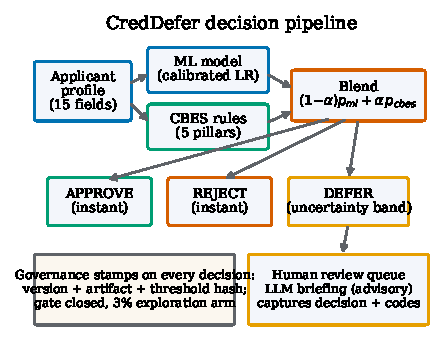
\includegraphics[width=\columnwidth]{figures/fig_architecture.pdf}
\caption{The CredDefer pipeline. Two independent opinions (a calibrated ML
model and the CBES rule engine) are blended; the blend decides instantly
outside an uncertainty band and defers inside it. Every decision carries
engine version, artifact name and a threshold-artifact hash; reviewer
outcomes are captured behind a closed relearning gate with a 3\%
exploration arm.}
\label{fig:arch}
\end{figure}

\textbf{Two opinions.} The serving ML model is a calibrated logistic
regression over a 15-field profile contract (holdout AUC 0.6919); the
contract guarantees the training-time derivation is byte-identical to the
live API's. CBES (Credit-Based Evaluation System) is a transparent rule
engine over five weighted pillars (credit, capacity, behaviour, liquidity,
stability) with a standalone AUC of 0.5650---deliberately an
\emph{explanation layer}, not a predictor.

\textbf{Blend and thresholds.} Decisions use
$p = (1-\alpha)\,p_{ml} + \alpha\,p_{cbes}$ with $\alpha = 0.10$ chosen from
a measured cost table on a tuning split, bounding CBES's influence to
$\pm 0.0075$ in probability. The base approve threshold ($t_{base}=0.65$) is
fitted by expected-cost minimisation, never on evaluation data; approve and
reject cutoffs bracket it, and the band between them defers.

\textbf{Capacity-aware deferral.} The deferral rate is a business constraint
(20--25\% underwriter capacity; we operate at 22.5\%), implemented as a
tuning-split quantile of the deferral signal. Section~\ref{sec:deferral}
evaluates \emph{which} signal deserves that budget.

\textbf{Capture without feedback.} Reviewer decisions, reason codes,
self-rated confidence and handling time are captured for governance analyses
(override-rate monitoring in the spirit of model-risk guidance), but no code
path reads them as training labels: a four-condition relearning gate is
evaluated on every inspection and has never opened, and a 3\% exploration arm
preserves the counterfactual labels any future relearning would require. We
treat the \emph{refusal} to close the loop as a design feature against
selective-labels feedback.

\textbf{Provenance.} Every decision is stamped with the engine version,
serving-artifact name, and a hash of the threshold artifact, surfaced in the
API, both dashboards, and the audit report.

\section{Evaluation Protocol}\label{sec:protocol}
All experiments share one discipline, fixed in each experiment script's
header before results existed. Data: the Home Credit application table
(307{,}511 rows, 8.07\% default rate, 14.3\% thin-file) plus its credit-bureau
table~\cite{homecredit}. Comparisons: 5-fold stratified cross-validation
(seed 42), identical folds across every experiment so deltas are
fold-paired. Claim rule: a gain is claimed only if the fold-paired mean AUC
delta exceeds $+0.0036$---the observed fold standard deviation---and, for
feature claims, every fold's delta is positive. Early stopping uses an inner
10\% split of training folds only. Policy quantities (thresholds,
calibrators, deferral cutoffs) are fitted on a 50/50 tuning split (seed
20260831) and reported on the held-out half. We use ROC-AUC as the model
criterion because at an 8\% default rate accuracy is dominated by the class
prior (always-approve scores 91.9\%); operating-point metrics are reported
only with their threshold stated.

\section{Results: Where Accuracy Lives}\label{sec:results}

\subsection{Features versus fusion}
We held models, folds, and metric fixed and changed only the features: v1,
the original $\sim$113-column numeric frame; v2, 319 engineered columns
adding domain ratios (payment burden, credit-to-annuity term proxy),
external-score combinations, and 35 deep aggregates of the full
credit-bureau table. Fig.~\ref{fig:folddeltas} shows the result:
\emph{all twenty} fold deltas are positive and every model's mean gain is at
least four times the noise floor, whereas the best honest fusion of the
improved models (a simple average of the three boosted ensembles) gains
$+0.0016$---real in direction (paired bootstrap CI $[0.0010, 0.0021]$) but
below the claim floor. Out-of-fold correlations among the improved models
remain 0.87--0.96: better features made every model better \emph{in the same
way}. A single-model gain attribution assigns 56\% of the top-25 gain
importance to the engineered features, led by the external-score mean
(30\%). Separately, a 14-configuration hyperparameter sweep over the boosted
ensembles improved the early-stopped default by $+0.001$---under a third of
the floor---and the capacity-adaptive learning curve
(Fig.~\ref{fig:learning}) still rises at full data ($+0.010$ AUC per
doubling): optimisation is converged, information is not.

\begin{figure}[t]
\centering
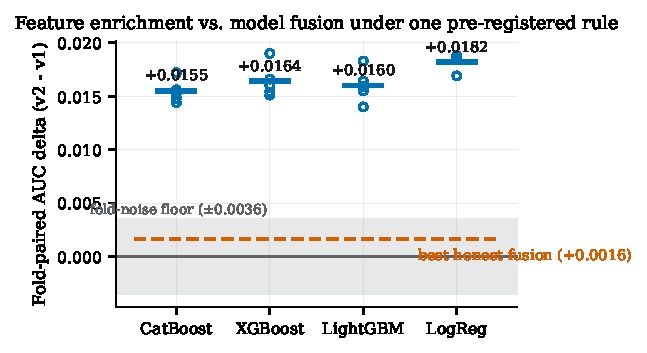
\includegraphics[width=\columnwidth]{figures/fig_fold_deltas.pdf}
\caption{One pre-registered rule judges both claims. Circles: per-fold AUC
deltas from feature enrichment (v2$-$v1), identical folds; bars: fold-paired
means. All 20 deltas clear the $\pm0.0036$ noise floor (shaded). The best
honest fusion of the improved models (dashed) does not.}
\label{fig:folddeltas}
\end{figure}

\begin{figure}[t]
\centering
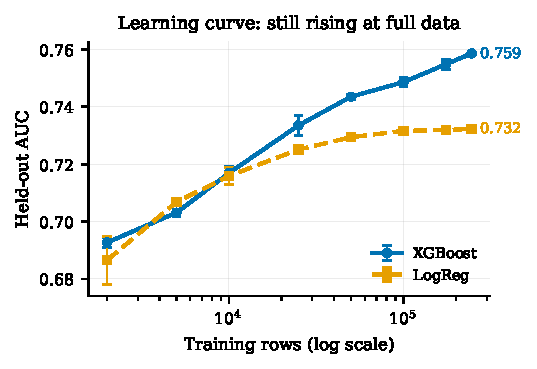
\includegraphics[width=\columnwidth]{figures/fig_learning_curve.pdf}
\caption{Capacity-adaptive learning curve (per-size early stopping; a fixed
tree budget underfits at scale and flattens the curve spuriously). The
boosted model still gains $\approx0.010$ AUC per data doubling at the full
246k training rows.}
\label{fig:learning}
\end{figure}

\subsection{Foundation models and 2026 challengers}
Table~\ref{tab:models} summarises every model evaluated under the protocol.
TabPFN-2.5 and Google TabFM~1.0 were scored on 8{,}000 rows joined by
applicant identity with an alignment gate (zero label mismatches; AUC
reproduces to four decimals)---a safeguard we added after an early
row-misalignment incident, and which we recommend as standard practice for
foundation-model comparisons. Both trail tuned gradient boosting; both
fusions die under the floor, and the TabFM average actively hurts
(CI $[-0.022, -0.007]$) despite TabFM being the most decorrelated partner we
ever tested ($\rho = 0.66$)---diversity obtained by being wrong does not
cancel errors. Among 2026 challengers screened under the same rules (30k
subsample, defaults only, advance on positive fold-paired delta), the
benchmark-tuned RealMLP lost every fold to CatBoost ($-0.0121$ fold-paired),
and TabICLv2 could not complete the screen on commodity hardware (its
in-context inference required $\sim$18\,GB of offload scratch per fold)---a
deployability result in itself. The TabPFN family's weights licences
(non-commercial, explicitly covering model \emph{outputs}) independently
preclude use in lending decisions; our screens therefore prioritised
permissively licensed challengers.

\begin{table}[t]
\centering
\caption{Models under one protocol. OOF = 5-fold out-of-fold on 307{,}511
rows; id-rows = 8{,}000 identity-verified rows; holdout = serving contract.}
\label{tab:models}
\begin{tabular}{@{}l l l@{}}
\toprule
\textbf{Model} & \textbf{AUC} & \textbf{Protocol} \\
\midrule
CatBoost + engineered features & \textbf{0.7757} & OOF \\
XGBoost + engineered features & 0.7749 & OOF \\
LightGBM + engineered features & 0.7721 & OOF \\
XGBoost (original features) & 0.7651 & OOF \\
Logistic regression (research) & 0.7560 & OOF \\
RealMLP-TD (2026 challenger) & 0.7360 & 30k screen \\
TabPFN-2.5 (Prior Labs) & $0.7284 \pm 0.0127$ & id-rows \\
Logistic regression (serving) & 0.6919 & holdout \\
Google TabFM 1.0 & $0.6911 \pm 0.0113$ & id-rows \\
CBES rule engine & 0.5650 & holdout \\
\bottomrule
\end{tabular}
\end{table}

\section{Results: Deferral Quality}\label{sec:deferral}

\subsection{Auditing a deployed router}
The original production rule deferred on raw score disagreement
$|p_{ml}-p_{cbes}| > \delta$. Measured on real out-of-fold predictions, the
two scores differ by a near-constant calibration offset (mean $+0.307$,
positive on 98.4\% of rows) that \emph{widens with model confidence}; the
rule therefore deferred the model's most confident cases. Against a
random-router null (200 permutations), the deferred pile's accuracy
signature sat at $z \approx +28\sigma$ on a held-out split---confident cases
systematically sent to humans. We propose this simple audit (deferred-pile
statistics versus a random router) as a deployment check for any L2D system.

\subsection{Repair and the single-model uncertainty signal}
Racing candidate signals at the mandated 22.5\% rate (thresholds from the
tuning split only), classical model-uncertainty routing in the serving
operating frame reversed the inversion to $z = -99.7$: the deferred pile
became genuinely harder than random. Beyond the repair, we evaluated
\emph{epistemic} uncertainty from a single SGLB-trained CatBoost
(posterior-sampling mode; $K{=}10$ virtual ensembles~\cite{malinin2021}),
whose decomposition separates knowledge uncertainty (mutual information)
from data uncertainty. At the matched rate on the test half
(Fig.~\ref{fig:riskcov}), knowledge uncertainty reached position 0.40 on the
random$\to$oracle axis versus 0.14 for the reject-option
baseline~\cite{chow1970} (selective risk 0.217 vs.\ 0.271; random 0.299),
and approached a two-model disagreement signal (0.47) \emph{without a second
model}. Knowledge uncertainty is also the only competitive signal not
reducible to the predicted probability itself (total-entropy signals
correlate 0.94 with $p$ at this base rate), and it is higher on thin-file
applicants, as an epistemic signal should be. In the serving frame, the
production default remains the repaired uncertainty rule; promoting the SGLB
signal is an explicitly versioned governance decision.

\begin{figure}[t]
\centering
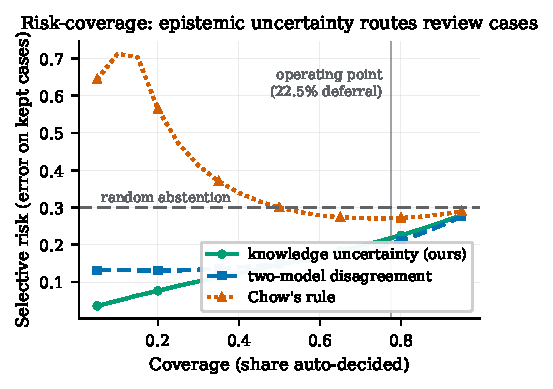
\includegraphics[width=\columnwidth]{figures/fig_risk_coverage.pdf}
\caption{Risk--coverage on the held-out half (research operating frame,
Youden threshold fitted on the tuning half). Single-model epistemic
(knowledge) uncertainty dominates the reject-option baseline at every
coverage and approaches two-model disagreement without a second model.}
\label{fig:riskcov}
\end{figure}

\section{Results: Pricing Compliance}\label{sec:studies}
\textbf{Monotonicity is free.} We fixed 21 sign constraints from domain
knowledge only (external credit scores decrease risk; payment burden, bureau
overdues, leverage and prolongations increase it; demographic fields
deliberately unconstrained) and re-trained the best model under them.
Fold-paired cost: $-0.0008$ AUC---inside the noise floor---with zero
direction violations in 14{,}400 empirical sweep checks. Directional
adverse-action explanations (``your bureau score improved, so your risk
decreased'') thus become \emph{model properties}, which is what the RBI
FREE-AI explainability posture asks for and post-hoc attribution alone
cannot guarantee~\cite{rbifreeai}.

\textbf{Cost-sensitivity belongs in the decision layer.} With a stated
7.5:1 false-negative:false-positive cost model (unsecured-retail loss-given-
default vs.\ forgone margin), class-weighted \emph{training} never beat
cost-optimal \emph{thresholding} of the unweighted model (test cost delta
$+0.000087$ per applicant; paired-bootstrap CI spans zero; the weighted arm
loses at four of five decision-time cost ratios)---an empirical confirmation
of Elkan's analysis~\cite{elkan2001} that justifies keeping the economics in
auditable decision policy rather than inside the model.

\section{Deployment}\label{sec:deploy}
CredDefer runs as a containerised service (FastAPI backend, React front-end,
model baked into the image) on commodity cloud infrastructure defined
end-to-end in Terraform: one small instance, a managed PostgreSQL database in
private subnets reachable only through security-group chaining, and a
container registry pulled via instance roles (no credentials on the
machine). The full stack rebuilds from nothing in $\sim$15 minutes and
destroys to zero cost; the demonstration database seeds itself with a
committed 510-customer sample spanning instant-approve, instant-reject and
defer outcomes. The TabPFN-2.5 second opinion---whose checkpoint and
in-context set exceed commodity GPU memory---is served from a free cloud GPU
behind an authenticated tunnel and consumed strictly as advisory input;
a \emph{connection run} validates the remote endpoint by scoring 400
locally-held labelled rows the remote never saw (last run: remote AUC 0.710,
within the model's known interval), so a mis-wired tunnel fails loudly
rather than silently. An LLM reviewer briefing (provider-pluggable)
summarises each deferred case from its decision report under three hard
boundaries: advisory only, optional by construction (absent credentials
degrade to an instructive 503), and grounded in the report with cited
fields. Operational lessons we believe generalise: cache governance
endpoints that recompute from large artifacts (a 36\,MB artifact recomputed
per request saturated a 1\,GB instance); treat boot-script changes as
instance replacements; and audit free-tier platform restrictions before
capacity planning.

\section{RBI Alignment}\label{sec:rbi}
Mapping to the Digital Lending Directions~\cite{rbi2025} and
FREE-AI~\cite{rbifreeai}: \emph{explainability} is served by per-decision
SHAP attributions, CBES pillar breakdowns, and the monotonicity guarantee of
Sec.~\ref{sec:studies}; \emph{human oversight} by capacity-aware deferral
with reviewer capture and override monitoring; \emph{auditability} by
provenance stamps (engine version, artifact, threshold hash) on every
decision and regeneration of all reported numbers from committed scripts;
\emph{model governance} by the versioned separation of research and serving
tracks and the closed relearning gate. We state one caveat openly: TabPFN-2.5
outperforms the deployed serving model on identical features (0.7446
best-case vs.\ 0.6919) and remains advisory because of its non-commercial
output licence, its GPU footprint, and the governance rule that advisory AI
never writes decisions; the roadmap is to promote the engineered-feature
gradient-boosted model behind the same serve-time contract.

\section{Limitations}
Our results are one-dataset (Home Credit; Indian-market cost and regulatory
framing, non-Indian data); the serving/research accuracy gap (0.6919 vs.\
0.7757) reflects a deliberate 15-field serve-time contract not yet extended
to the engineered features; deferral findings are reported in two operating
frames (serving and research) whose baselines differ, and the SGLB routing
result, while pre-registered, awaits production promotion; the committed
demonstration sample under-represents the extreme-risk tail (we corrected
this by appending identity-verified reject-tail applicants); and the
relearning loop is deliberately unproven because it is deliberately closed.

\section{Conclusion}
Treating the decision pipeline---not the classifier---as the research object
yielded reproducible findings a leaderboard cannot express: on this corpus,
accuracy headroom lives in information rather than architecture; deferral
rules can silently invert and can be audited with a one-line permutation
test; a single boosted model can supply calibrated epistemic routing without
an ensemble; and a regulator's explainability guarantee can be had for free.
Future work: the unused credit-history side tables (a measured
$\sim$$+0.015$ AUC path), promotion of the engineered-feature model behind
the serving contract, and domain-hosted deployment enabling full
identity-provider integration.

\section*{Reproducibility}
All experiments are committed scripts writing machine-readable reports; every
number above traces to one. Code, infrastructure definitions, figure
generators and reports are available from the authors.
% TODO(authors): insert repository URL if/when the repo is made public or an
% anonymised archive is prepared.

\begin{thebibliography}{25}

\bibitem{rbi2025} Reserve Bank of India, ``Reserve Bank of India (Digital
Lending) Directions,'' Mumbai, India, 2025.

\bibitem{rbifreeai} Reserve Bank of India, ``Framework for Responsible and
Ethical Enablement of Artificial Intelligence (FREE-AI): Committee Report,''
Mumbai, India, 2025.

\bibitem{homecredit} Home Credit Group, ``Home Credit Default Risk,'' Kaggle
competition dataset, 2018. [Online]. Available:
\url{https://www.kaggle.com/c/home-credit-default-risk}

\bibitem{chow1970} C. K. Chow, ``On optimum recognition error and reject
tradeoff,'' \emph{IEEE Trans. Information Theory}, vol. 16, no. 1, pp.
41--46, 1970.

\bibitem{madras2018} D. Madras, T. Pitassi, and R. Zemel, ``Predict
responsibly: Improving fairness and accuracy by learning to defer,'' in
\emph{Advances in Neural Information Processing Systems (NeurIPS)}, 2018.

\bibitem{mozannar2020} H. Mozannar and D. Sontag, ``Consistent estimators for
learning to defer to an expert,'' in \emph{Proc. Int. Conf. Machine Learning
(ICML)}, 2020.

\bibitem{mao2023} A. Mao, M. Mohri, and Y. Zhong, ``Two-stage learning to
defer with multiple experts,'' in \emph{Advances in Neural Information
Processing Systems (NeurIPS)}, 2023.

\bibitem{dearteaga2020} M. De-Arteaga, R. Fogliato, and A. Chouldechova, ``A
case for humans-in-the-loop: Decisions in the presence of erroneous
algorithmic scores,'' in \emph{Proc. CHI Conf. Human Factors in Computing
Systems}, 2020.

\bibitem{lakshminarayanan2017} B. Lakshminarayanan, A. Pritzel, and C.
Blundell, ``Simple and scalable predictive uncertainty estimation using deep
ensembles,'' in \emph{Advances in Neural Information Processing Systems
(NeurIPS)}, 2017.

\bibitem{mukhoti2023} J. Mukhoti, A. Kirsch, J. van Amersfoort, P. H. S.
Torr, and Y. Gal, ``Deep deterministic uncertainty: A new simple baseline,''
in \emph{Proc. IEEE/CVF Conf. Computer Vision and Pattern Recognition
(CVPR)}, 2023.

\bibitem{guo2017} C. Guo, G. Pleiss, Y. Sun, and K. Q. Weinberger, ``On
calibration of modern neural networks,'' in \emph{Proc. Int. Conf. Machine
Learning (ICML)}, 2017.

\bibitem{malinin2021} A. Malinin, L. Prokhorenkova, and A. Ustimenko,
``Uncertainty in gradient boosting via ensembles,'' in \emph{Proc. Int.
Conf. Learning Representations (ICLR)}, 2021.

\bibitem{angelopoulos2023} A. N. Angelopoulos and S. Bates, ``Conformal
prediction: A gentle introduction,'' \emph{Foundations and Trends in Machine
Learning}, vol. 16, no. 4, pp. 494--591, 2023.

\bibitem{gibbs2021} I. Gibbs and E. Cand\`es, ``Adaptive conformal inference
under distribution shift,'' in \emph{Advances in Neural Information
Processing Systems (NeurIPS)}, 2021.

\bibitem{geifman2017} Y. Geifman and R. El-Yaniv, ``Selective classification
for deep neural networks,'' in \emph{Advances in Neural Information
Processing Systems (NeurIPS)}, 2017.

\bibitem{lundberg2017} S. M. Lundberg and S.-I. Lee, ``A unified approach to
interpreting model predictions,'' in \emph{Advances in Neural Information
Processing Systems (NeurIPS)}, 2017.

\bibitem{ribeiro2016} M. T. Ribeiro, S. Singh, and C. Guestrin, ``\,`Why
should I trust you?' Explaining the predictions of any classifier,'' in
\emph{Proc. ACM SIGKDD Int. Conf. Knowledge Discovery and Data Mining},
2016.

\bibitem{wachter2017} S. Wachter, B. Mittelstadt, and C. Russell,
``Counterfactual explanations without opening the black box: Automated
decisions and the GDPR,'' \emph{Harvard Journal of Law \& Technology},
vol. 31, no. 2, 2018.

\bibitem{elkan2001} C. Elkan, ``The foundations of cost-sensitive
learning,'' in \emph{Proc. Int. Joint Conf. Artificial Intelligence
(IJCAI)}, 2001.

\bibitem{hollmann2025} N. Hollmann, S. M\"uller, L. Purucker, A.
Krishnakumar, M. K\"orfer, S. B. Hoo, R. T. Schirrmeister, and F. Hutter,
``Accurate predictions on small data with a tabular foundation model,''
\emph{Nature}, vol. 637, pp. 319--326, 2025.

\bibitem{chen2016} T. Chen and C. Guestrin, ``XGBoost: A scalable tree
boosting system,'' in \emph{Proc. ACM SIGKDD Int. Conf. Knowledge Discovery
and Data Mining}, 2016.

\bibitem{ke2017} G. Ke et al., ``LightGBM: A highly efficient gradient
boosting decision tree,'' in \emph{Advances in Neural Information Processing
Systems (NeurIPS)}, 2017.

\bibitem{prokhorenkova2018} L. Prokhorenkova, G. Gusev, A. Vorobev, A. V.
Dorogush, and A. Gulin, ``CatBoost: Unbiased boosting with categorical
features,'' in \emph{Advances in Neural Information Processing Systems
(NeurIPS)}, 2018.

\end{thebibliography}

\end{document}
